\section{Shepard JS}
\label{research:ShepardJS}
\textbf{Source:} \cite{ShepherdjsDocs}
Having showed a few peers my project and had the same questions asked of me by each I knew that I needed a system to help introduce users to the basic philosophies of my project. Whilst I have researched thoroughly and be careful to make my software intuitive to all by definition of reinventing a commonly done task (in this case notetaking) there has to be some instruction to users regarding how my implementation differs. Firstly I explored a variety of methods for introducing users namely: Video tutorials, Documentation and guided tours.

From personal experience I knew very few users would read through a 'wall of text' to use some software and would likely just switch back to their familiar options (which I do not want), Whilst I might still write some documentation for complex 'pro' features the tutorial at least should avoid it. This left video tutorials and guided tours. Whilst I do frequently actively search for help on platforms such as YouTube I was sceptical to their benefits for the users first experience. Much like documentation it leaves the user watching the steps required rather than being actively involved in the learning process. This left guided tours as my best option and upon reflecting on my competitor analysis at the start of the project I found that the most successful 'onboarding' utilised an interface tour at their centre.

With the concept in mind I now looked to the technical implementation. A web search revealed three options to me: Vue-Tour, Tourguide Js and Shepsard Js. Whilst all three seemed to serve the same function, through looking at their documentation and demos I found Shepard Js to be the most logical in its approach and whilst the default aesthetic wasn’t particularly pleasing to me, it was highly customisable and I could modify to fit my needs. With a framework now chosen I spent an hour or so reading through the documentation \cite{ShepherdjsDocs} and began planning the tour process.

I chose to have the tour trigger when a user signs in and has 0 notes In their graph, this would ensure all new users would have the option of the tour and that users who perhaps made an account long ago but were only now coming back to the tour had the same opportunity presented to them, I also made the tour accessible from a clear button in the user dropdown menu.

Through my research of other applications tours I found that the most successful formula was to focus on the interface elements the user will see, explaining what they do and how they link in to the wider philosophy of the note taking app in question, with this in mind I planned out my user tour 'flow':

\begin{longtable}{%
        >{\centering\arraybackslash}p{1.5cm}
    >{\raggedright\arraybackslash}p{0.316\textwidth}
    >{\raggedright\arraybackslash}p{0.316\textwidth}
    >{\raggedright\arraybackslash}p{0.316\textwidth}
    }


    \caption{User tour flow}                                                                                                                                                     \\
    \toprule
    \textbf{Step} & \textbf{Title?}       & \textbf{Content}                                                                                              & \textbf{Progression} \\
    \midrule
    \endfirsthead

    \toprule
    \textbf{Step} & \textbf{Title?}       & \textbf{Content}                                                                                              & \textbf{Progression} \\
    \midrule
    \endhead

    \midrule
    \multicolumn{3}{r}{\emph{Continued on next page}}                                                                                                                            \\
    \bottomrule
    \endfoot

    \bottomrule
    \endlastfoot

    % === Table content begins ===
    0             & Welcome to NeuroNote! & Let's take a quick tour to get you started with your knowledge management system.                             & Start tour button    \\
    1             & Navigation sidebar    & This is your main navigation sidebar where you can manage all your tabs and navigate between different views.

    • Collapse or expand the sidebar for more screen space
    • Create new tabs and organize your workspace
    • Switch between different types of content
    Quick tip: Use Cmd/Ctrl + / to quickly toggle the sidebar!
                  & Next button                                                                                                                                                  \\
   2 & Tab shortcuts 
 & Here you can find some quick tab shortcuts for easy navigation around your workspace.

• Click any shortcut to quickly open that section
• Use the search button to find specific notes and tags
 Power user tip: Use Cmd/Ctrl + J to instantly search through all your notes and tags! & Next button

    \\
    3 & Profile &

This dropdown gives you access to your profile, settings, and other important features.

• Access your profile and account settings
• Give feedback and access Legal documents
• Find quick actions and help resources
Come back anytime: You can restart this tour from the help section in this menu!
&
Next button \\

4 &

Active Tab &

This is where the magic happens! When you open a tab, it will show up here, showing you exactly what you are working on.

Right now we're on the dashboard tab - let's explore what it offers!

Navigation tip: You can switch between tabs using the sidebar &

Next button \\
5 &

Recent Notes &

This section shows your most recent notes. You can click on any of these to open them directly in a new tab. &

Next button \\

6 &

Shortcuts &

Here you can configure some shortcut buttons for quick access to your most used notes and tags. You can add, remove, or rearrange them as you like.

• Click the pencil icon to edit your shortcuts
• Give them a fun, descriptive name
• Add your favorite notes and tags for instant access
 Productivity boost: Create shortcuts for your most important content to save time! &

Next button \\
7 &

Note graph &

Ready to be amazed? Your note graph visualizes connections between notes, tags, and ideas. As you create content, you'll see your knowledge network grow here.

It might look empty now, but let's add some structure to it!

• Watch connections form as you link notes and tags
• Use filters to find exactly what you need, and spotlight to highlight the details
• Click on any element to open it directly
• If you fancy a change of scenery just press shuffle and watch the engine create beautiful layouts
 Knowledge mapping: This visual representation helps you find your notes and discover unexpected connections between your ideas! &

Next button \\

8 &

Create your first tag &

1. Click the + New button in the toolbar above the graph

2. Select Tag from the dropdown menu

3. Give your tag a name (e.g. "My First Tag")

Quick tip: You can also press T as a shortcut!
The tour will automatically continue once you create your tag &

/auto on tag creation/  OR skip step button \\

9 &

Create your first note &

You've created your first tag! Now you can start connecting it to notes and other tags. This will help you build a rich knowledge graph over time lets make a note
1. Click the + New button again

2. Select Document from the dropdown

3. Give your note a name

Magic moment: Since you have a tag selected, the note will automatically connect to it!
The tour continues automatically when you create the note &

/auto on note creation/ OR skip step button \\

10 &

Great Job! &

With a note created you can see how it connects to the graph - if you want to make more connections later you can drag the red dot from a note to a tag or select from the dropdown in the note editor.

Deleting a connection is just as easy - simply hold down on the connecting line and drag to delete.

1. Click on your note in the graph to open it in a new tab
 Pro tip: You can also click \& hold on any element for additional options!
The tour continues automatically when you open the note &

/auto on note open/ OR skip this step \\

11 &

Document Editor &

Welcome to the Document Editor! This is where you can write and format your notes using rich text formatting.

Let's explore what makes this editor so powerful!&

Next button \\

12 & 

Toolbar &

The toolbar provides quick access to formatting options and note history &

Next button \\
13 &

Main Content Area &

This is your main content area where you can write and format your note. You can start typing right away and use many helpful shortcuts including:

• Use - for bullet points
• Use 1. for numbered lists
• Use \# to add headings
and so many more

Pro tip: Type / while writing to see a menu of formatting options and special blocks! &

Next button \\

14 &

Content Linking &

Earlier you may have noticed the option to create a whiteboard rather than a document. While documents are great for formatting beautiful typed notes, whiteboards excel at letting your creativity flourish!

They're perfect for brainstorming, mind mapping, and sketching out ideas. You can easily integrate both by attaching whiteboard previews to your notes.

1. Type the / command in the editor
2. Start typing "whiteboard"
3. Click the whiteboard option when it appears
Magic trick: This seamlessly blends visual and text-based thinking in one note!
The tour continues automatically when the whiteboard popup opens &

/auto on whiteboard popup open/ OR skip step button \\

15 &

Select whiteboard &

In this popup you can select an existing whiteboard or create a new one. As we haven't made one yet, let's create a new one.

1. Type a name for your whiteboard
2. Click the "Create" button
Auto-magic: The new whiteboard will automatically be added to your knowledge graph!
The tour continues automatically when the whiteboard is created &

/auto on whiteboard created/ OR skip step button \\

16 &

Whiteboard Preview &

Great! You now have a whiteboard attached to your note. You may notice it's looking a little blank - let's fix that! 

1. Click the edit button in the top right to open it in a new tab and start sketching out your ideas
Visual thinking: This is a powerful way to visualize your thoughts and connect them to your notes!
The tour continues automatically when you open the whiteboard editor &

/auto on whiteboard editor opening/ OR skip step button \\

17 &

Whiteboard Editor &

Welcome to the Whiteboard Editor! This is where you can draw, sketch, and brainstorm your ideas.

Let's explore what makes this editor so powerful!

• Use various tools to create shapes and draw freehand
• Add images and text to enhance your sketches
• All your changes are saved automatically
Creative freedom: Perfect for visual thinking, mind maps, and bringing your ideas to life! &

Next button \\
18 &

Toolbar &
The toolbar provides quick access to drawing tools and whiteboard controls.

• Switch between auto, draw, and select input modes
• Adjust pen controls like color and thickness
• Access shapes, text, images, and other drawing tools
• View whiteboard history and undo changes
 Smart switching: Auto mode detects whether you're using a stylus or mouse and switches tools accordingly! &

Next button \\

19 &

Main Content Area &

This is your main content area where you can see the whiteboard you just created. You can start creating right away!

• Use the pen tool to draw freehand
• Select shapes and images from the toolbar
• Drag and resize elements to organize your ideas
Start creating: Your whiteboard is ready - let your creativity flow! &

Next button \\

20 &

Congratulations! &

That's it for the tour! You've learned the basics of NeuroNote, including how to create notes, tags, and whiteboards.

You now have all the tools you need to build your personal knowledge management system!

• Access this tour again from your profile menu
• Find help resources in the profile dropdown
• Share feedback through the feedback form
 Ready to start: Begin building your knowledge network and let your ideas flourish!
Happy note-taking!  &

Finish Tour \\

    % === Table content ends ===
\end{longtable}

With my tour steps planned out I focused on implementation.
I first wrote the styling code to change the look of each step from stock to my custom Design
\begin{figure}[H]
    \centering
    \begin{minipage}{0.48\textwidth}
        \centering
        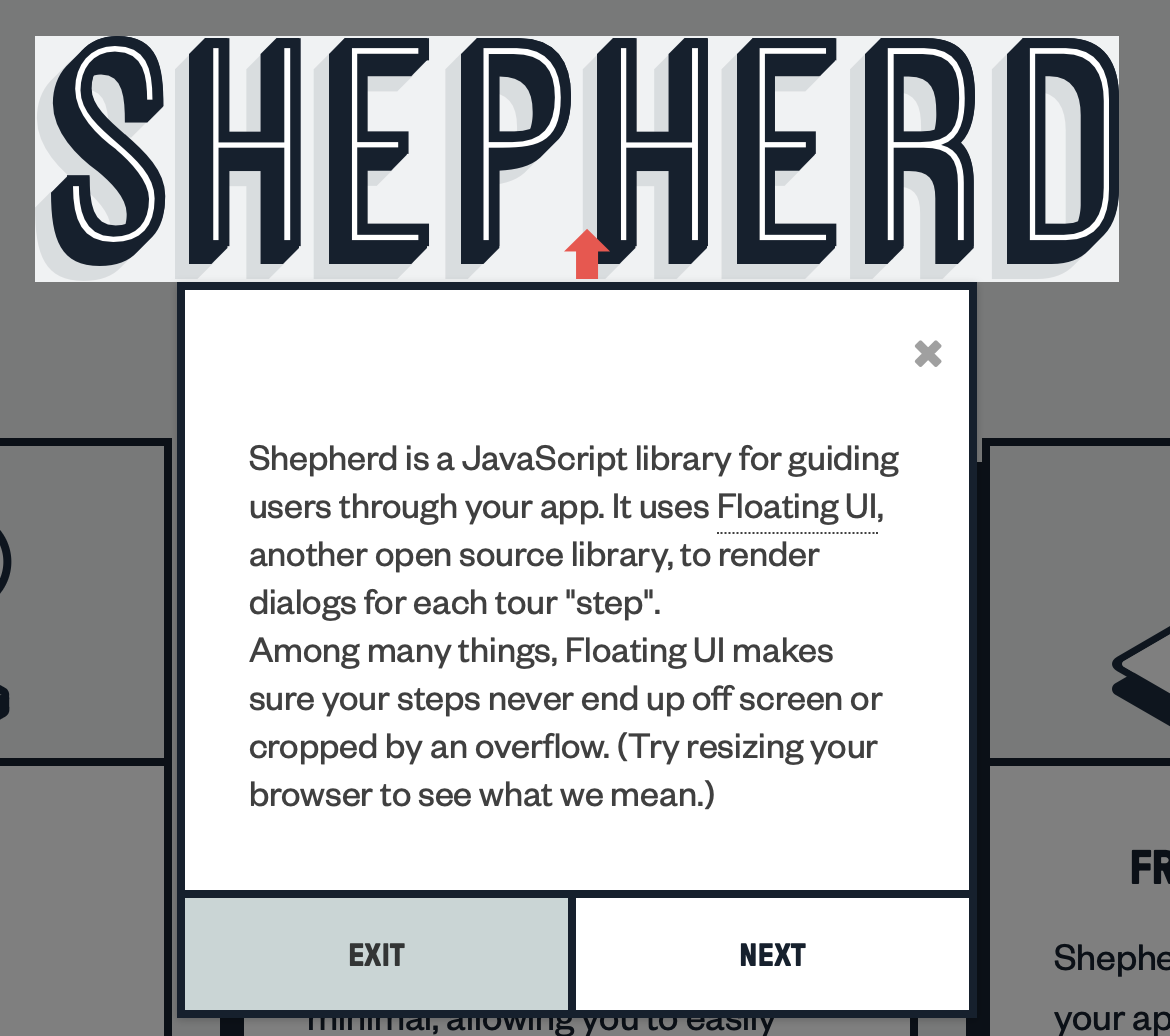
\includegraphics[width=\linewidth]{Research/29_ShepardJS/media/defaultStyle.png}
        \caption{Default Shepherd JS styling}
        \label{fig:shepherdjs-default}
    \end{minipage}\hfill
    \begin{minipage}{0.48\textwidth}
        \centering
        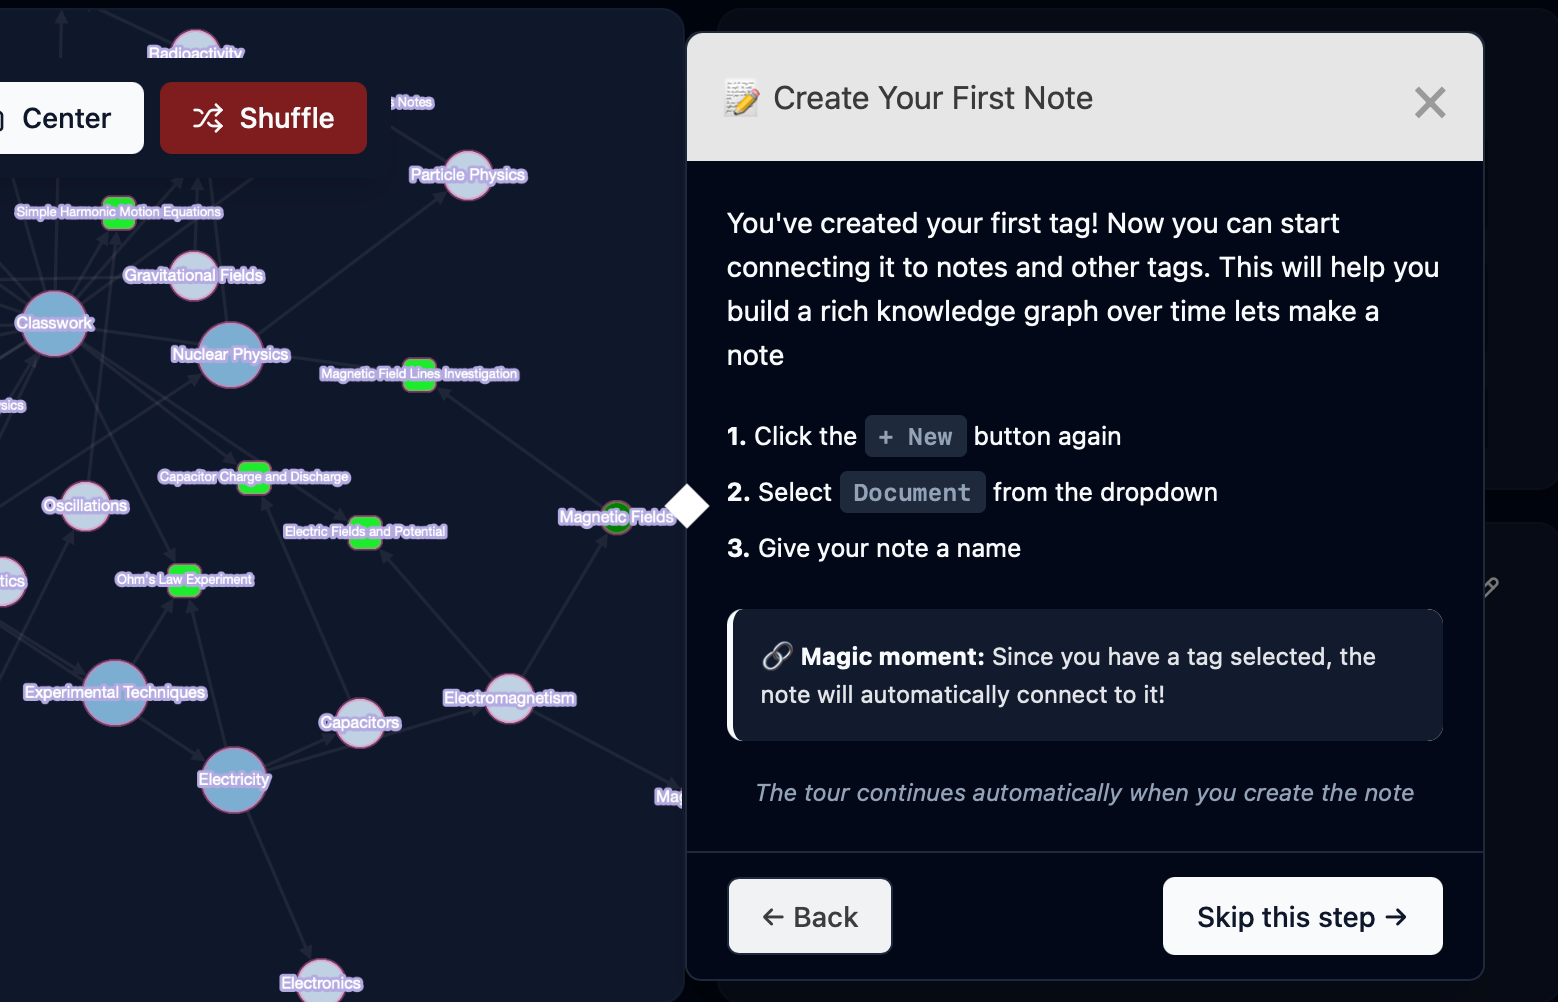
\includegraphics[width=\linewidth]{Research/29_ShepardJS/media/customStyle.png}
        \caption{Custom NeuroNote tour styling}
        \label{fig:shepherdjs-custom}
    \end{minipage}
\end{figure}

Next I coded the structure of the tour, showing the steps in a linear order and making them progress once the user completes the required action (if applicable), to make the auto progression function I had to build a number of 'flags' into the respective components so that the tour could recognise that e.g. a tag was created. I also ensured the user could easily go back to a prior step and that the tour was accessible to screen readers and could be controlled using arrow keys / specialist devices such as braille keyboards. I debated whether to add a progression bar to the interface however from some A/B testing (how the test felt with vs without the progress bar) with family I found that they were more likely to skip steps to 'race to finish' when the progress bar was there and that without that information they felt the tour was subjectively faster hence I do not include one.

Finally I added the above content into the tour, tested on a variety of platforms to ensure it worked nicely on different screen sizes and light/dark mode, and merged the finished code into my main project.

\begin{figure}[H]
    \centering
    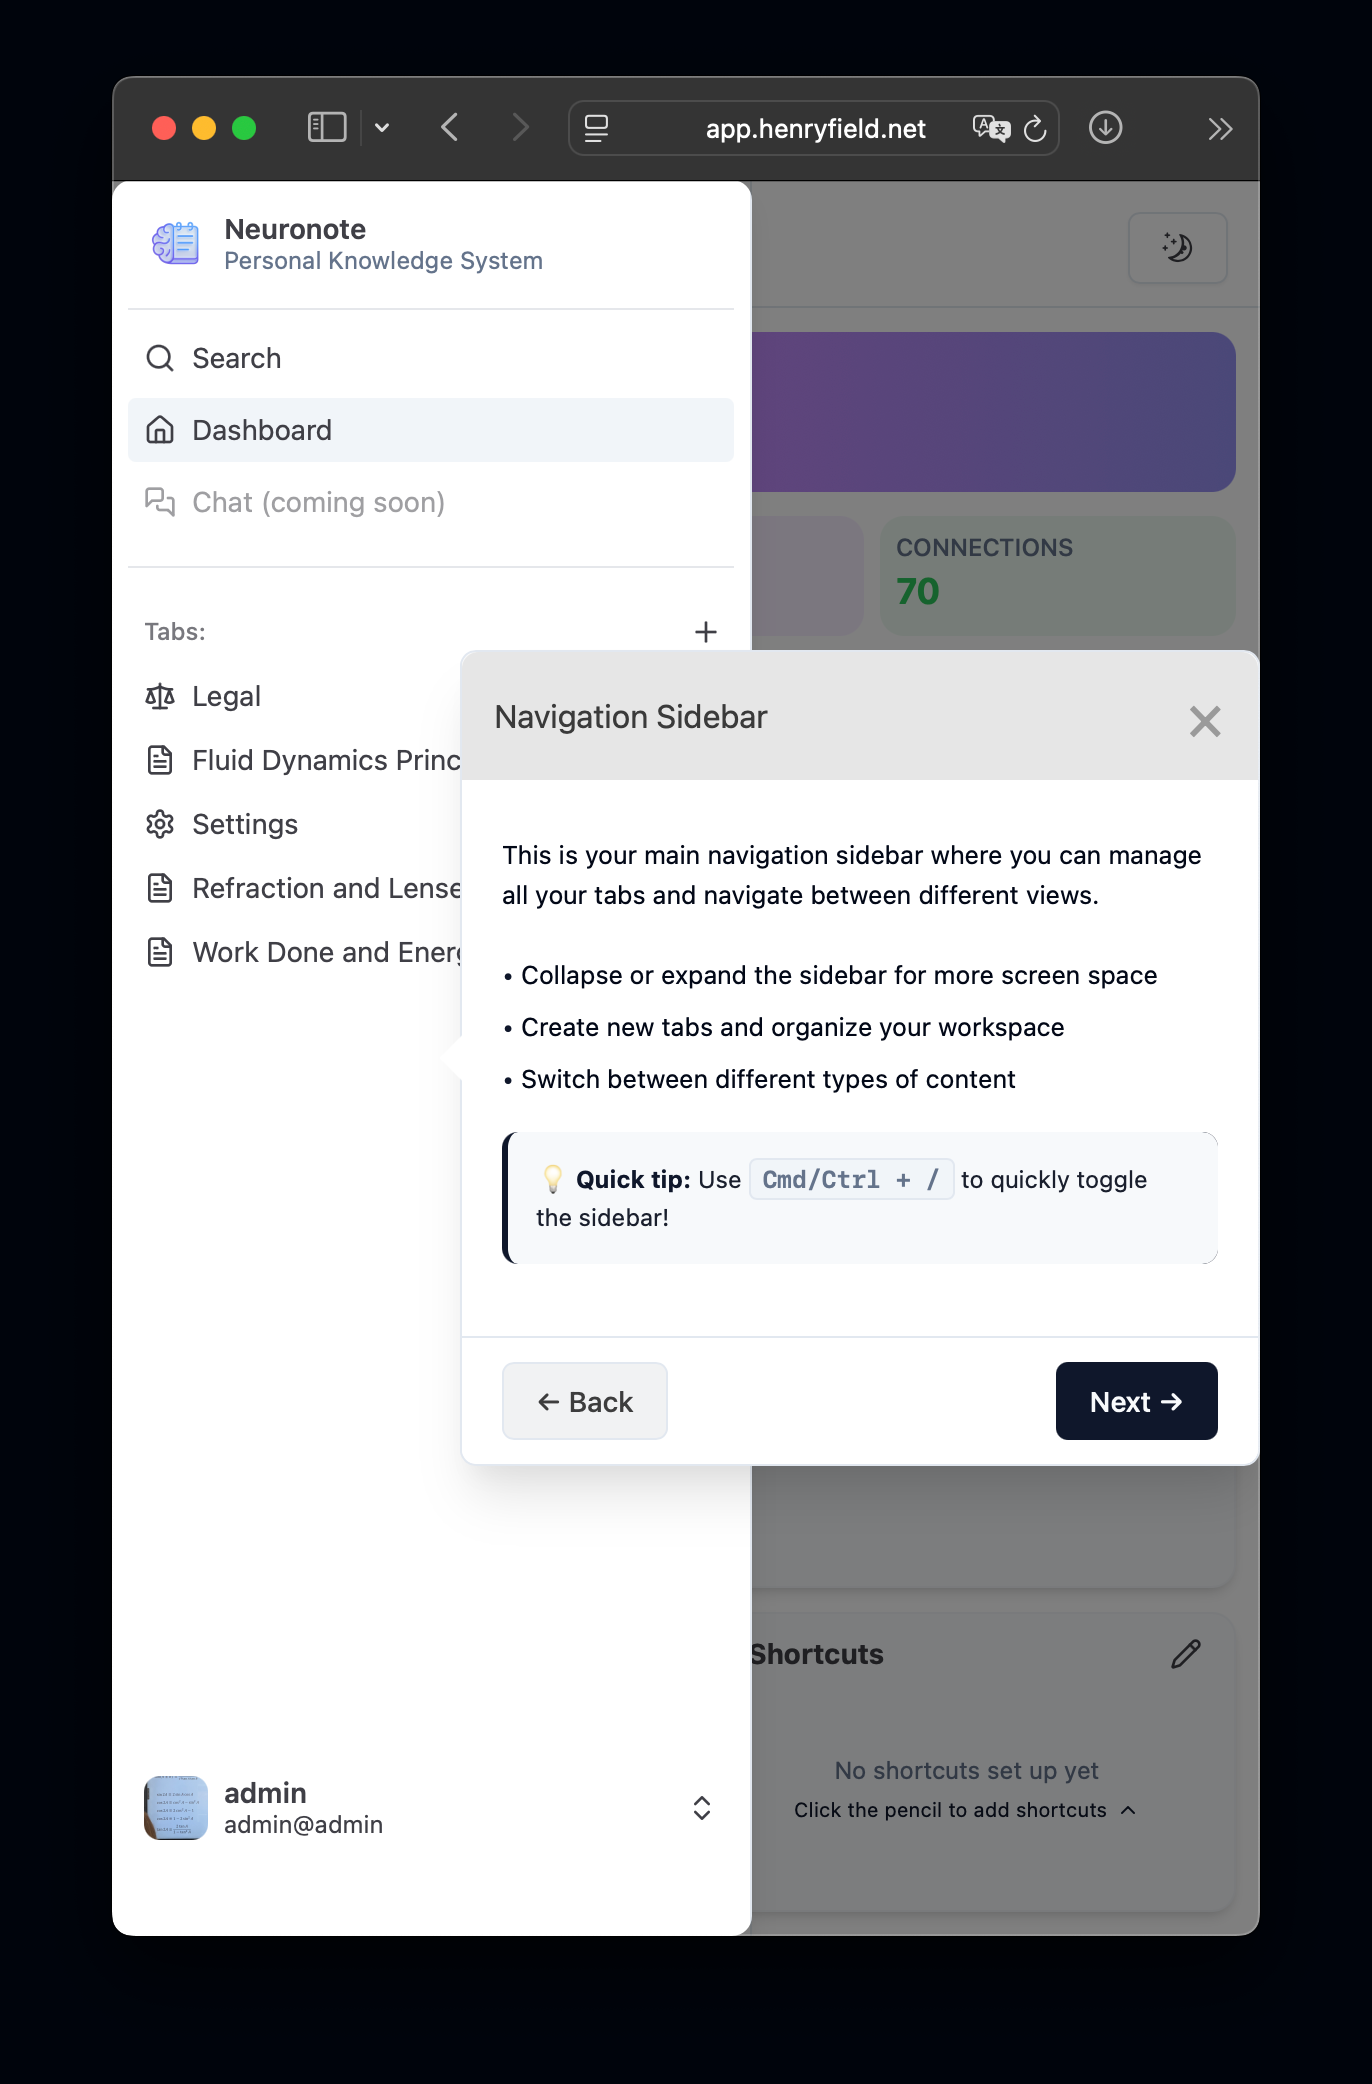
\includegraphics[width=0.8\linewidth]{Research/29_ShepardJS/media/mobileStyle.png}
    \caption{Mobile style of Shepard JS tour}
    \label{fig:shepherdjs-demo}
\end{figure}

The most challenging screen size - mobile, makes the tour automatically pop open the sidebar so that the relevant steps can accurately points to the correct interface element irrespective of the users screen size.